\section{Overview}

\section{Component View}

\subsection{Database}
The application database will be managed using a Relational DBMS.
It allows the reading of data, ensuring users the ability to log in and access the applications of interest and check the stored data.
It is also used for data manipulation (insertion, modification and deletion).
The use of a Relational DBMS guarantees the fundamental properties for a database of this type:
\begin{itemize}
  \item Atomicity: no partial executions of operations.
  \item Consistency: the database is always in a consistent state.
  \item Isolation: each transaction is executed in an isolated and independent way.
  \item Durability / Persistence: changes made are not lost.
\end{itemize}
The database will offer to the Application Server an interface that it can use to interact with the database.
The data stored in the database must be considered personal and confidential, therefore, procedures must be implemented to safeguard the stored information.
Particular attention must be paid to the reading permissions granted to users and to the encryption of passwords used to access the services offered.
Below is the designed E-R diagram:

\begin{figure}[H]
  \begin{center}
  	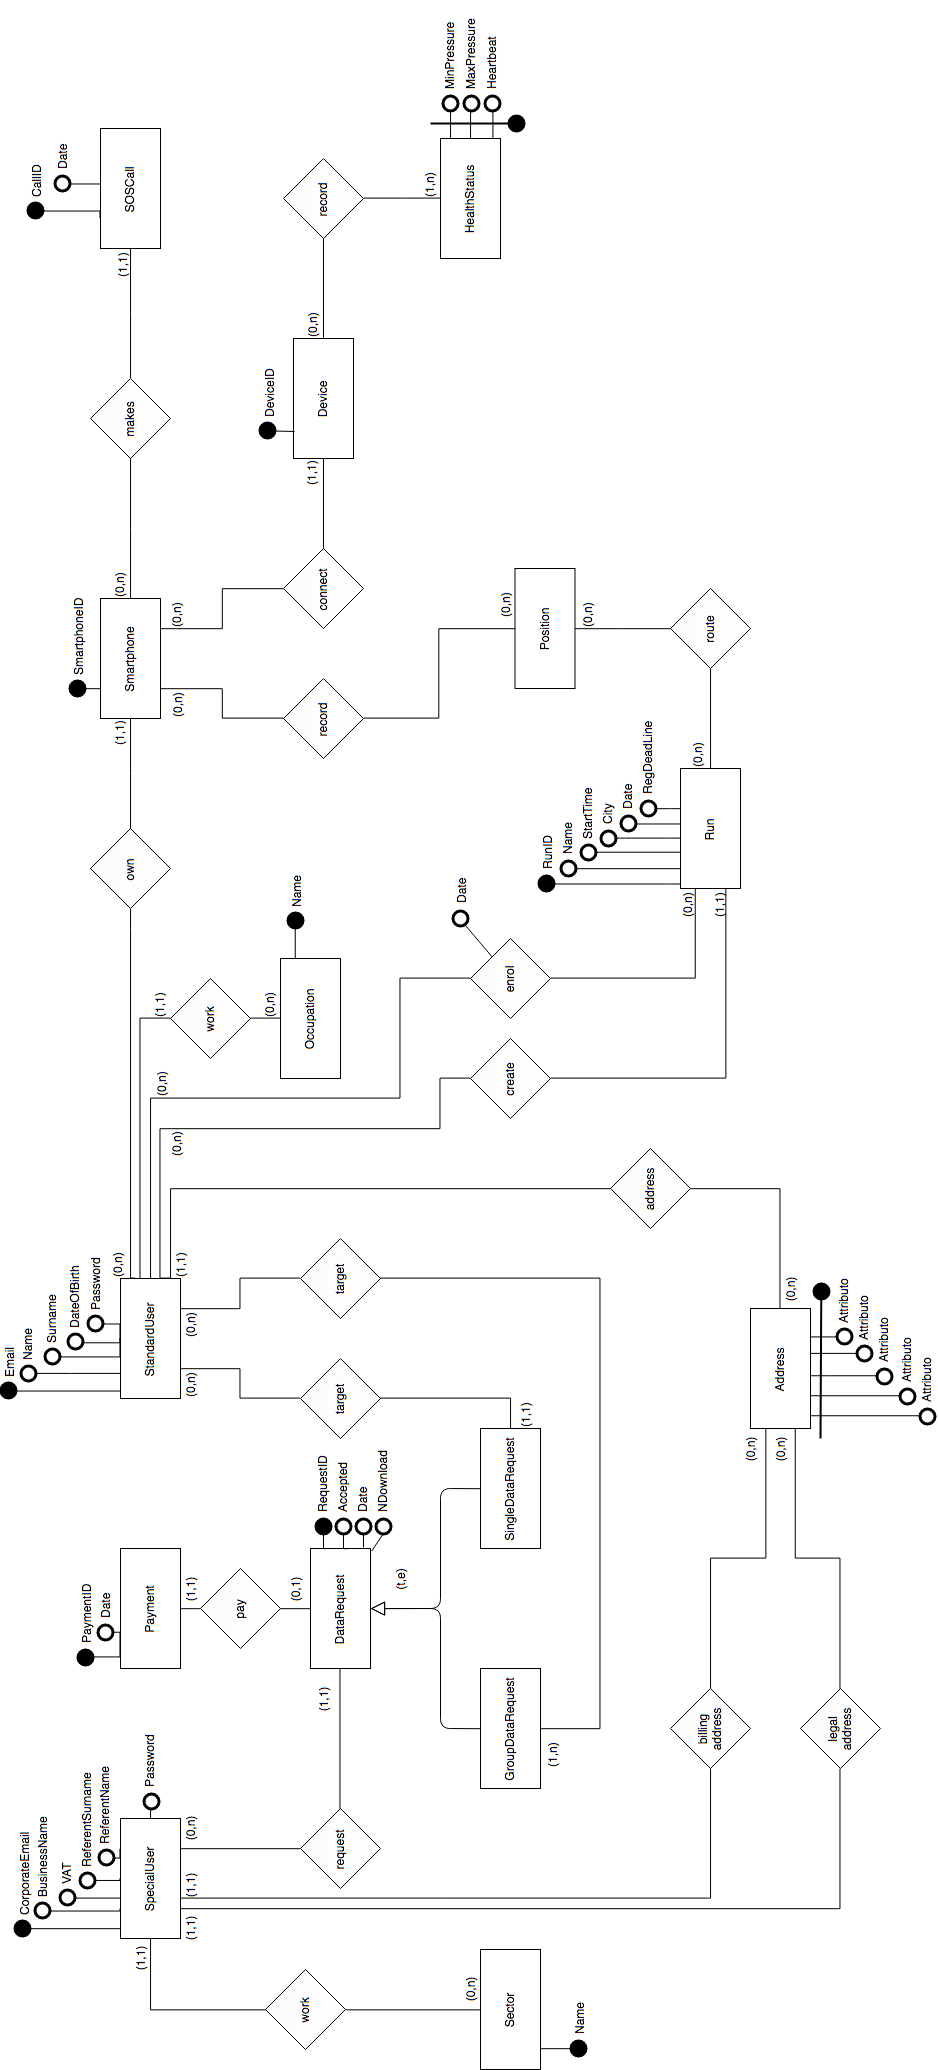
\includegraphics[width=\textwidth,height=0.58\paperheight,keepaspectratio]{./img/ER.png}
		\caption{\textit{E-R} Diagram.}
    \hspace{0.05\linewidth}
    \centering
		\label{img:ER Diagram}
    \end{center}
\end{figure}

\section{Deployment View}

\section{Runtime View}

\section{Component Interfaces}

\section{Selected Architectural Styles and Patterns}

\section{Other Design Decisions}
